% ==============================================================================================
\chapter{One-dimensional wave propagation in an elastic column with an absorbing boundary} \label{ch:one_dim_abs_boundary}
% ==============================================================================================

% ----------------------------------------------------------------------------------------------
\section{Introduction}
% ----------------------------------------------------------------------------------------------
This benchmark compares the STEM numerical solution against the analytical solution,
for the one dimensional wave propagation in a vertical elastic soil column with an absorbing boundary at the bottom,
subjected to a surface load.

The analytical solution for 1D wave propagation on infinite columns is presented in~\cite{Verruijt_2010}.
The analytical solution provides closed-form expressions for the vertical velocity along the column,
enabling a direct time-history comparison against the numerical model.

% ----------------------------------------------------------------------------------------------
\section{Model Description}
% ----------------------------------------------------------------------------------------------

% ..............................................................................................
\subsection{Geometry, mesh and loading}
% ..............................................................................................
Two soil domains are modelled, a two-dimensional and a three-dimensional continuum representing vertical columns.
The two-dimensional column is modelled with a height of \qty{10}{\meter} and a width of \qty{0.25}{\meter}.
The three-dimensional column is modelled with a height of \qty{10}{\meter} and a square cross-section of
\qty{0.25}{\meter} by \qty{0.25}{\meter}.
The columns are aligned with the $y$-axis, so that wave propagation is essentially one-dimensional along
the vertical direction.

For the two-dimensional column, the soil is discretised with second-order triangular elements, for the three-dimensional
column, the soil is discretised with second-order tetrahedral elements.
In both cases, an average element size of \qty{0.10}{\meter} is adopted.
An overview of the geometries and meshes adopted for the analysis is shown in
Figure~\ref{fig:one_dim_wave_abs_mesh}.
A vertical distributed load is applied on the entire top face of the column. The load acts in compression along
the $y$-direction and is applied as a step function in time:

\begin{equation}
	p(t) =
	\begin{cases}
		0, & t < \qty{0}{\second}, \\
		\qty{-1000}{\kilo\newton\per\meter\squared}, & t \geq \qty{0}{\second}.
	\end{cases}
\end{equation}

The base of the column has an absorbing boundary condition, absorbing all waves in the normal direction.
In the two-dimensional case, the side lines are restrained in the horizontal direction.
In the three-dimensional case, the four vertical faces are restrained only in the horizontal directions,
thereby allowing vertical motion similar to a one-dimensional situation.

\begin{figure}
	\centering
	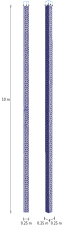
\includegraphics[width=0.2\textwidth]{one_d_abs_boundary/one_d_column_mesh.pdf}
	\caption{Geometry and mesh adopted for the one-dimensional
	wave propagation with absorbing boundary benchmark. }
	\label{fig:one_dim_wave_abs_mesh}
\end{figure}

% ..............................................................................................
\subsection{Materials and numerical parameters}
% ..............................................................................................
The soil is modelled as a one-phase continuum with a linear elastic constitutive law, with the
following parameters:

\begin{itemize}[noitemsep,topsep=0pt,parsep=0pt,partopsep=0pt]
	\item Young's modulus: \qty{50}{\mega\pascal},
	\item Poisson ratio: \qty{0.3}{},
	\item Solid density: \qty{2700}{\kilogram\per\meter\cubed},
	\item Porosity: 0.3.
\end{itemize}


Material damping is included via Rayleigh damping, with parameters that provide a damping ratio of
\qty{0.5}{\percent} at \qty{1}{\hertz} and \qty{80}{\hertz}.

The dynamic analysis is performed over a \qty{0.20}{\second} time window, with a time step of \qty{0.001}{\second}.
The system of equations is solved using the Newmark time integration~\cite{Newmark_1959} scheme with
parameters $\beta = 0.25$ and $\gamma = 0.5$.


% ----------------------------------------------------------------------------------------------
\section{Results}
% ----------------------------------------------------------------------------------------------
Figure~\ref{fig:one_dim_wave_abs_boundary_results} presents the time histories of the
vertical velocity at a point located at:  \qty{2.5}{\meter}, \qty{5}{\meter} and \qty{7.5}{\meter}
along the height of the column.
The figure compares the numerical STEM results against the analytical solution of the one-dimensional wave equation with
absorbing boundary.

The arrival time of the incident wave at the observation point matches closely between the numerical
and analytical solution. It can also be observed that there is no reflection from the bottom boundary,
indicating that the absorbing boundary condition is functioning as intended.
The amplitude of the velocity pulse also shows very good agreement.

\begin{figure}[h]
	\centering
	\includegraphics[width=0.8\textwidth]{one_d_abs_boundary/time_history.pdf}
	\caption{Comparison of the vertical velocity time history at \qty{5}{\meter} along the column height.}
	\label{fig:one_dim_wave_abs_boundary_results}
\end{figure}
